\chapter{Introduzione}
Si richiamano brevemente alcuni concetti sugli operatori differenziali che risulteranno la base per le discussioni successive. L'operatore fondamentale è $\nabla$, che in coordinate cartesiane è definito come
\begin{equation}
    \nabla := \bigg(\frac{\p}{\p x},\frac{\p}{\p y},\frac{\p}{\p z}\bigg).
\end{equation}
Questo operatore compare nelle definizioni delle operazioni di gradiente, divergenza e rotore. 

Il gradiente è l'applicazione dell'operatore $\nabla$ ad una funzione $f(x,y,z)$, per cui 
\begin{equation}
    \rem{grad}(f) \equiv \nabla f = (\p_xf)\h{i} + (\p_yf)\h{j} + (\p_zf)\h{k} \equiv 
    \begin{pmatrix}
        \p_xf \\
        \p_yf \\
        \p_zf
    \end{pmatrix}.
\end{equation}
La nozione di gradiente può in generale essere interpretata come un operatore che aumenta di uno il rango dell'oggetto a cui viene applicato; ad esempio, applicando considerando il gradiente $A_i$ si ottiene un tensore, infatti
\begin{equation}
    (\nabla A)_{ij} = \p_iA_j.
\end{equation}

Dall'altra parte, la divergenza può essere vista come il prodotto scalare tra l'operatore $\nabla$ e un vettore, per cui 
\begin{equation}
    \rem{div}(\v{A}) \equiv \nabla \cdot \v{A} = \p_iA_i.
\end{equation}
dove si è usata la notazione di Einstein per gli indici ripetuti\footnote{Nel seguito non si distinguerà mai tra indici covarianti e controvarianti.}. La nozione di divergenza può in generale essere interpretata come un operatore che diminuisce di uno il rango dell'oggetto a cui viene applicato; ad esempio, considerando la divergenza di un tensore $T_{ij}$ si ottiene un vettore, infatti
\begin{equation}
    (\nabla \cdot T)_i = \p_jT_{ij}.
\end{equation}

Invece, il rotore può essere definito, a differenza di gradiente e divergenza, solo per i vettori e può essere visto come il prodotto vettoriale tra l'operatore $\nabla$ e il vettore, per cui
\begin{equation}
    \begin{aligned}
        \rem{rot}(\v{A}) \equiv \nabla \times \v{A} = 
        \begin{vmatrix}
            \h{i} & \h{j} & \h{k} \\
            \p_x & \p_y & \p_z \\
            A_x & A_y & A_z
        \end{vmatrix} &= (\p_yA_z - \p_zA_y)\h{i} + (\p_zA_x - \p_xA_z)\h{j} \\
        &+ (\p_xA_y - \p_yA_x)\h{k}.
    \end{aligned}
\end{equation}
Esistono poi innumerevoli identità vettoriali utili per semplificare i calcoli che si svolgeranno nel seguito; non si riportano qui, ma si farà riferimento al formulario in \cite{NRLPlasmaFormulary}.

Nel seguito, si userà prevalentemente il sistema di misura c.g.s invece che il più familiare Sistema Internazionale. Questo sistema risulta essere conveniente in quanto le uniche unità di misura presenti sono il grammo $\rem{g}$, il centimetro $\rem{cm}$ e il secondo $\rem{s}$, con le quali si possono costruire tutte le altre unità di misura presenti nel SI. Ad esempio, la carica elettrica fondamentale è misurata in 
\begin{equation}
    e = \SI{4.8e-10}{\rem{Fr}},
\end{equation}
dove $\rem{Fr}$ è lo ``stat Coulomb'' il quale è definito come 
\begin{equation}
    [\rem{Fr}] = \sqrt{\frac{\rem{g}\cdot\rem{cm}^3}{\rem{s}}}.
\end{equation}

\section{Prime nozioni sul plasma}
Lo stato solido è quello stato della materia dove i legami molecolari sono molto forti permettendo il mantenimento di una struttura rigida, Alzando la temperatura, tali legami vengono ad indebolirsi fino a che non sono abbastanza deboli da permettere alle molecolare di ``scivolare'' l'una sull'altra, passando dallo stato solido a quello liquido. Alzando ancora di più la temperatura, i legami continuano ad indebolirsi rendendo sempre più libere le molecolare di muoversi, passando allo stato gassoso. Ora, alzando ancora la temperatura le molecole del gas acquisteranno un'energia cinetica sempre maggiore, intorno ai $\SI{5000}{\celsius}$, si presenta il fenomeno della ionizzazione. Essenzialmente, la probabilità che gli elettroni degli atomi del gas vengano strappati da essi non diventa più trascurabile e pertanto all'interno del gas si generano delle forze di interazione elettriche, a causa della carica intrinseca delle particelle presenti, e magnetiche, dovute al fatto che tali particelle cariche si muovono nello spazio. Basandosi su questo, si può quindi dare una prima definizione di plasma:
\begin{quote}
    ``il plasma è l'emissione delle cariche elettriche e dei campi da esse generati''.
\end{quote}
A livello microscopico, che per le scale astrofisiche corrispondono al range tra i chilometri e le centinaia di chilometri, si studiano i plasmi tramite la teoria cinetica, mentre alle scale macroscopiche lo si fa tramite la teoria fluida e, successivamente, tramite la magnetoidrodinamica (MHD).

\subsection{Grado di ionizzazione}
Un aspetto fondamentale dei sistemi di plasmi sono le collisioni. Si consideri un atomo con una data sezione d'urto $\sigma_c$, Nell'unità di tempo $\tau$, l'atomo traccia un percorso cilindrico che determina la regione con cui altre particelle possono interagire con l'atomo. Supponendo quindi che all'interno di tale cilindro ci siano $\Delta N$ particelle, la densità di queste ultime è data da $n = \Delta N/\Delta V$, dove $\Delta V$ è il volume del cilindro. Le su dimensioni però sono note in quanto la base è $\sigma_c$ è l'altezza è la distanza percorsa nel tempo $\tau$ dall'atomo a velocità $v$, per cui
\begin{equation}
    \Delta V = \sigma_c v\tau = \frac{\Delta N}{n}.
\end{equation}
Si definisce quindi il libero cammino medio $\lambda$ come la distanza che l'atomo deve percorrere, in media, affinché interagisca con $\Delta N$ particelle, ossia
\begin{equation}
\label{eq: libero cammino medio}
    \lambda := \frac{v\tau}{\Delta N} = \frac{1}{\sigma_c n}.
\end{equation}
La definizione \eqref{eq: libero cammino medio} appare sensata in quanto $\lambda$ decresce all'aumentare di $\sigma_c$ e all'aumentare di $n$ contemporaneamente. In maniera simile, si può definire la frequenza di collisioni $\nu_c$ come
\begin{equation}
\label{eq: frequenza di collisioni}
    \nu_c := \frac{v}{\lambda} = n\sigma_c v.
\end{equation}

Ci si potrebbe ora chiedere, data la definizione di plasma, quale sia la soglia di ionizzazione affinché si possa considerare un sistema come un plasma. In altre parole, ci si chiede quante particelle devono essere ionizzate affinché il sistema sia descrivibile come un plasma. Per rispondere, si parte dalla seguente equazione del moto
\begin{equation}
\label{eq: equazione del moto degli elettroni}
    m_e\frac{d\v{v}}{dt} = -e\v{E} - m_e\nu_c\v{v}.
\end{equation}
Si noti che l'equazione del moto \eqref{eq: equazione del moto degli elettroni} contiene esclusivamente termini relativi agli elettroni. In linea di principio, si potrebbe considerare anche il contributo dei nuclei atomici; tuttavia, la massa degli elettroni è 2000 volte minore di quella di questi ultimi, pertanto possiedono un'inerzia minore e il loro contributo cinetico è maggiore di quello dei nuclei, dando origine alla quasi totalità della dinamica del sistema. La semplificazione principale che si è effettuata in \eqref{eq: equazione del moto degli elettroni} in realtà è la scelta di trascurare, per il momento, le interazioni magnetiche. Quindi, supponendo di essere a regime, ossia che $\p_t\v{v} = 0$, dall'equazione del moto si trova che
\begin{equation}
    \v{v} = -\frac{e\v{E}}{m_e\nu_c}.
\end{equation}
Introducendo ora la densità di corrente $\v{j} = -en_e\v{v}$, si può scrivere che
\begin{equation}
    \v{j} = \frac{e^2n_e}{m_e\nu_c}\v{E},
\end{equation}
dove si può identificare la conducibilità $\sigma$ presente nella legge di Ohm $\v{j} = \sigma\v{E}$, come 
\begin{equation}
    \sigma = \frac{e^2n_e}{m_e\nu_c}.
\end{equation}
Adesso è importante distinguere tra le possibili collisioni che possono avvenire. Tra tutte le possibilità, ci si concentra su quelli più rilevanti, ossia gli urti tra elettrone ed atomo ionizzato e quelli tra elettrone ed atomo neutro. In questo modo, la frequenza di collisione può essere separata in due termini
\begin{equation}
    \nu_c = \nu_c^{(ion)} + \nu_c^{(atom)} \equiv \nu_{c,i} + \nu_{c,a}.
\end{equation}
Ricordando poi la definizione della frequenza di collisioni in \eqref{eq: frequenza di collisioni}, si definisce $\alpha_x = \sigma_c\v{v}_x$, con $x = \{i,a\}$, così da avere 
\begin{equation}
    \nu_c = \alpha_in_i + \alpha_an_a = \alpha_in_i\bigg(1 + \frac{\alpha_an_a}{\alpha_in_i}\bigg).
\end{equation}
Si introduce poi il grado di ionizzazione $\chi$ come
\begin{equation}
    \chi := \frac{n_i}{n_a + n_i},
\end{equation}
da cui si può facilmente dedurre che è definito come un numero tale che $\chi \in [0,1]$, dove per $\chi = 0$ si intende un sistema completamente privo di ioni, mentre per $\chi = 1$ si intende un sistema completamente ionizzato. Usando la definizione di $\chi$, si può riscrivere $\nu_c$ come
\begin{equation}
    \nu_c = \alpha_in_i\bigg(1 + \frac{\alpha_a}{\alpha_i}\frac{1 - \chi}{\chi}\bigg),
\end{equation}
con la quale si può scrivere la conducibilità $\sigma$ come
\begin{equation}
    \sigma = \frac{e^2n_e}{m_e\alpha_in_i}\bigg(1 + \frac{\alpha_a}{\alpha_i}\frac{1 - \chi}{\chi}\bigg)^{-1}.
\end{equation}
Dato che in generale $n_e = Zn_i$, si ha
\begin{equation}
    \sigma = \frac{Ze^2}{m_e}\bigg(\alpha_i + \alpha_a\frac{1 - \chi}{\chi}\bigg)^{-1} \equiv \frac{\sigma_{max}}{1 + \dfrac{\alpha_a}{\alpha_i}\dfrac{1 - \chi}{\chi}},\quad \sigma_{max} \equiv \frac{Ze^2}{m_e\alpha_i},
\end{equation}
dove $\sigma_{max}$ è il valore massimo della conducibilità, ovvero per $\chi = 1$. Tipicamente, la sezione d'urto della collisione elettrone-ione è molto più grande di quella della collisione tra elettrone ed atomo neutro, in particolare
\begin{equation}
    \frac{\alpha_a}{\alpha_i} \simeq 10^{-2},
\end{equation}
implicando un andamento di $\sigma$ consistente in una crescita molto rapida in funzione di $\chi$, come mostrato in figura \ref{fig: conducibilità plasma}. Dalla figura si nota come sia sufficiente che $\chi = 0.2$ per avere una conducibilità pari al 90\% di $\sigma_{max}$, anche solo per $\chi = 10^{-2}$ si ha una conducibilità pari al 50\% di $\sigma_{max}$. 
\begin{figure}[ht]
    \centering
    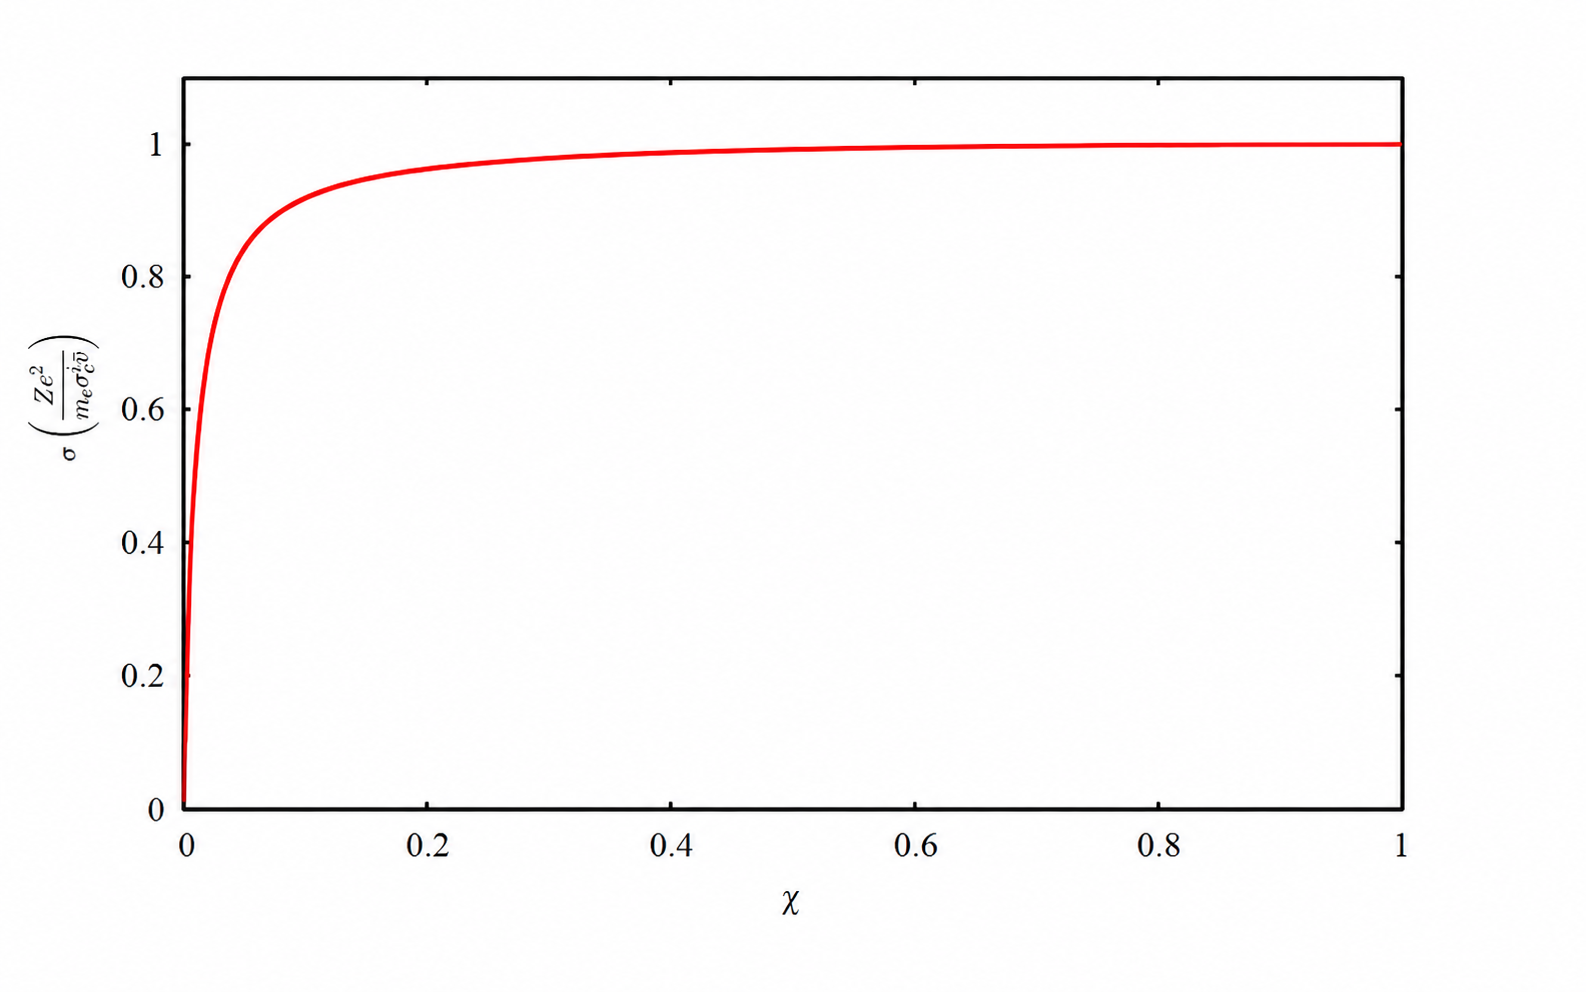
\includegraphics[width=0.65\linewidth]{Immagini - Capitolo 1/conducibilita' plasma.png}
    \caption{andamento di $\sigma$ in funzione di $\chi$.}
    \label{fig: conducibilità plasma}
\end{figure}

Si consideri adesso un gas composto da idrogeno. Per ionizzare un singolo atomo di idrogeno sono necessari $\SI{13.6}{\eV}$, ma questo è vero solo alla temperatura di $\SI{e5}{\celsius}$. Ci si potrebbe quindi chiedere come sia possibile che si possano avere plasmi a temperature di molto inferiori a questo valore. La risposta sta nella definizione di temperatura. Quest'ultima è un concetto statistico, non tutti gli atomi che compongono il gas hanno la medesima energia cinetica: la maggior parte avrà un'energia cinetica vicina al valore medio della distribuzione, ma alcuni avranno valori molto più piccoli o molto più grande del valore medio. Gli atomi responsabili dell'esistenza di plasmi anche a temperature minori di $\SI{e5}{\celsius}$ sono proprio quella piccola percentuale di atomi con un'energia cinetica molto maggiore del valore medio, in quanto, come visto prima, è sufficiente un minimo grado di ionizzazione per avere una conducibilità elettrica elevata, ossia per avere uno stato di plasma.

\subsection{Equazione di Saha}
L'equazione di Saha descrive il grado di ionizzazione di un plasma come una funzione della temperatura, della densità e dell'energia di ionizzazione degli atomi. L'equazione è
\begin{equation}
\label{eq: equazione di Saha}
    \frac{n_{k + 1}n_e}{n_k} = \frac{2}{\Lambda^3}\frac{g_{k + 1}}{g_k}\exp{\bigg(-\frac{E_{k + 1} - E_k}{kT}\bigg)},\quad \Lambda \equiv \sqrt{\frac{h^2}{2\pi m_ekT}},
\end{equation}
dove $n_k$ è la densità di atomi allo stato $k$-esimo, $g_k$ è il fattore di ionizzazione, $E_k$ è l'energia necessaria per rimuovere $k$ elettroni dall'atomo neutro e $\Lambda$ è la lunghezza di de Broglie termica. Dalla definizione di $E_k$, si deduce che la differenza $E_{k + 1} - E_k$ in \eqref{eq: equazione di Saha} corrisponde all'energia necessaria per rimuovere il $(k + 1)$-esimo elettrone. 

Ad esempio, per l'idrogeno, considerando $k = 0$ come stato fondamentale e $k = 1$ come lo stato di ionizzazione, l'equazione \eqref{eq: equazione di Saha} porta a
\begin{equation}
    \frac{n_1n_e}{n_0} \equiv f(T) \simeq (2.4 \times 10^{15})\times T^{3/2}\exp{\bigg(\frac{-1.58\times 10^5}{T}\bigg)},
\end{equation}
con $2g_1/g_0 = 1$. Per un gas di idrogeno però $n_i = n_e$, per cui usando $n_i = \chi n_t$ con $n_t = n_i + n_0$, si può scrivere $n_0 = n_t - n_i = n_t(1 - \chi)$, da cui
\begin{equation}
    \frac{n_in_e}{n_0} = \frac{\chi^2n_t^2}{n_t(1 - \chi)} = f(T),
\end{equation}
che si può riscrivere come l'equazione di secondo grado
\begin{equation}
    \chi^2 n_t + \chi f(T) - f(T) = 0,
\end{equation}
la quale ha soluzione
\begin{equation}
    \chi = \frac{2f(T)}{f(T) + \sqrt{f(T)^2 + 4f(T)}},
\end{equation}
dove si è selezionata la soluzione con $\chi > 0$ dato che $\chi \in [0,1]$.
\begin{figure}[h]
    \centering
    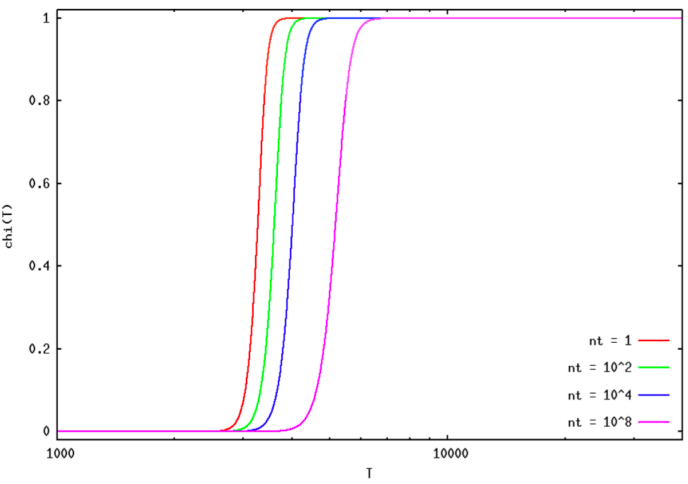
\includegraphics[width=0.65\linewidth]{Immagini - Capitolo 1/grado di ionizzazione (eq. saha).png}
    \caption{grado di ionizzazione $\chi$ in funzione di $T$ per diversi valori di $n_t$.}
    \label{fig: grado di ionizzazione (eq. saha)}
\end{figure}

\section{Schermatura di Debye}
Si consideri un reticolo di cariche positive e negative disposte in maniera omogenea, cosicché il sistema sia complessivamente neutro. Si supponga ora di introdurre una carica di prova $q_T$ con carica negativa. Questo inserimento provoca una perturbazione del sistema modificando la distribuzione di carica attraendo a sé le cariche positive e respingendo quelle negative. Il sistema complessivamente continua ad essere neutro, tuttavia, a seconda della distanza a cui si osserva la carica $q_T$, la carica misurata non sarà nulla. 

Si intende quindi determinare la distanza dalla quale il sistema torna ad essere complessivamente neutro. Per farlo, si parte dall'equazione di Maxwell per il campo elettrico
\begin{equation}
    \nabla \cdot \v{E} = 4\pi q = 4\pi(n_i - n_e)e + 4\pi q_T\delta(\v{r}).
\end{equation}
Sapendo che $\v{E} = -\nabla\phi$, dove $\phi(r)$ è il potenziale elettrostatico, si può scrivere
\begin{equation}
    -\nabla^2\phi = 4\pi(n_i - n_e)e + 4\pi q_T\delta(\v{r}).
\end{equation}
Inoltre, la densità di ioni si può parametrizzare tramite $\phi(r)$ con
\begin{equation}
    n_i = n_0\exp{\bigg(-\frac{e\phi(r)}{kT}\bigg)},
\end{equation}
e in maniera simile, la densità di elettroni con
\begin{equation}
\label{eq: densità di elettroni}
    n_e = n_0\exp{\bigg[-\frac{(-e)\phi(r)}{kT}\bigg]},
\end{equation}
ottenendo quindi
\begin{equation}
    -\nabla^2\phi = 4\pi en_0\bigg[\exp{\bigg(-\frac{e\phi(r)}{kT}\bigg)} - \exp{\bigg(-\frac{(-e)\phi(r)}{kT}\bigg)}\bigg] + 4\pi q_T\delta(\v{r}).
\end{equation}
Si assume ora che $e\phi(r)/kT \ll 1$. In questo modo, è possibile espandere l'equazione appena ricavata in serie di Taylor, così da avere
\begin{equation}
    \begin{split}
        \nabla^2\phi &= -4\pi n_0e\bigg(1 - \frac{e\phi(r)}{kT} - 1 - \frac{e\phi(r)}{kT}\bigg) - 4\pi q_R\delta(\v{r}) \\
        &= \frac{8\pi e^2n_0}{kT}\phi(r) - 4\pi q_R\delta(\v{r}).
    \end{split}
\end{equation}
Assumendo una distribuzione di carica sferica, è conveniente scrivere il laplaciano in coordinate sferiche\supcite[6]{NRLPlasmaFormulary} così da avere
\begin{equation}
    \frac{1}{r^2}\p_r[r^2\p_r\phi(r)] = \frac{8\pi e^2n_0}{kT}\phi(r) - 4\pi q_R\delta(\v{r}).
\end{equation}
Usando l'analisi dimensionale, si riscrive l'equazione appena precedente in modo che ogni termine abbia la dimensione $[\rem{potenziale}/L^2]$, per cui 
\begin{equation}
\label{eq: equazione del potenziale elettrostico in coordinate sferiche}
    \frac{1}{r^2}\p_r[r^2\p_r\phi(r)] = \frac{\phi(r)}{\lambda_D^2} - 4\pi q_R\delta(\v{r}),
\end{equation}
dove $\lambda_D$ è la lunghezza di Debye, definita come 
\begin{equation}
\label{eq: lunghezza di Debye}
    \lambda_D := \sqrt{\frac{kT}{8\pi n_0e^2}}.
\end{equation}
Si assume ora che soluzione dell'equazione \eqref{eq: equazione del potenziale elettrostico in coordinate sferiche} sia la somma della soluzione per l'equazione con presente solo la carica $q_T$, a cui si associa il potenziale $\phi_T(r) =q_T/r$, e di quella dell'equazione dove $\phi(r) = \phi_T(r)f(r)$ dove $f(r)$ è una funzione radiale. Quindi, si hanno
\begin{equation}
    \begin{cases}
        \nabla^2\phi_T(r) = -4\pi q_T\delta(\v{r}) \\[2ex]
        \nabla^2(\phi_T(r)f(r)) = \dfrac{\phi_T(r)f(r)}{\lambda_D^2} - 4\pi q_T\delta(\v{r})
    \end{cases};
\end{equation}
facendo la differenza tra la seconda e la prima equazione si ottiene
\begin{equation}
    \begin{split}
        \frac{\phi_T(r)f(r)}{\lambda_D^2} &= \frac{1}{r^2}\p_r\{r^2\p_r[\phi_T(r)f(r) - \phi_T(r)]\} \\
        \frac{q_Tf(r)}{r\lambda_D^2} &= \frac{q_T}{r^2}\p_r\bigg[r^2\p_r\bigg(\frac{f - 1}{r}\bigg)\bigg] \\
        \frac{1}{r\lambda_D^2} &= \frac{1}{r^2}\p_r\bigg[r^2\bigg(-\frac{f - 1}{r^2} + \frac{1}{r}\p_rf(r)\bigg)\bigg] \\
        &= \frac{1}{r^2}\p_r[1 - f(r) + r\p_rf(r)] \\
        &= \frac{1}{r^2}[-\cancel{\p_rf(r)} + \cancel{\p_rf(r)} + r\p_r^2f(r)] \\
         &= \frac{1}{r^2}\p_r^2f(r).
    \end{split}
\end{equation}
Quindi, l'equazione si riduce a
\begin{equation}
    \p_r^2f(r) = \lambda_D^{-2},
\end{equation}
la cui soluzione è 
\begin{equation}
    f(r) = f_0\exp{\bigg(-\frac{r}{\lambda_D}\bigg)},
\end{equation}
dove si è scelta la soluzione con esponente negativo in quanto altrimenti si avrebbe $f(r) \to \infty$ per $r \to \infty$ e quindi un potenziale divergente. Necessariamente poi $f_0 = 1$ dato che in assenza di altre cariche oltre $q_T$ si deve ritornare al potenziale $\phi_T(r)$. Dunque, il potenziale completo è
\begin{equation}
\label{eq: potenziale elettrostatico Debye shielding}
    \phi(r) = \phi_Tf(r) = \frac{q_T}{r}\exp{\bigg(-\frac{r}{\lambda_D}\bigg)}.
\end{equation}
Questa modifica data da $f(r)$ al potenziale elettrostatico della carica libera è chiamata \emph{Debye shielding}, o schermatura di Debye.

Si deve ora giustificare la scelta iniziale $e\phi(r)/kT \ll 1$ da cui di fatto deriva tutta la derivazione per arrivare all'equazione \eqref{eq: potenziale elettrostatico Debye shielding}. Per farlo, si considera che per descrivere il sistema si è implicitamente seguito un approccio secondo la Meccanica statistica, la quale è una teoria accurata se la distanza media $\b{d}$ tra le particelle è molto minore di $\lambda_D$. La distanza media si può dedurre segua una legge del tipo $\b{d} \propto n^{-1/3}$ con $\b{d} \ll \lambda_D$. Combinando le due espressioni si ha che 
\begin{equation}
    \lambda_D^3n \gg 1,
\end{equation}
dove $\lambda_D^3n$ è di fatto il numero di particelle. Si calcoli ora l'argomento dell'esponenziale in equazione \eqref{eq: densità di elettroni} sulla distanza media usando l'equazione \eqref{eq: potenziale elettrostatico Debye shielding}, quindi si ha
\begin{equation}
    \frac{e\phi(r)}{kT}\bigg|_{r = \b{d}} = \frac{e^2}{kT\b{d}}\exp{\bigg(-\frac{\b{d}}{\lambda_D}\bigg)} \simeq \frac{e^2}{kT\b{d}} \propto \frac{e^2}{kT}n^{1/3} \simeq \bigg(\frac{\b{d}}{\lambda_D}\bigg)^2.
\end{equation}
Pertanto, dato che $b{d}/\lambda_D \ll 1$, allora l'assunzione iniziale che $e\phi(r)/kT \ll 1$ è legittima.
\begin{obs}
    Il fatto che la lunghezza di Debye $\lambda_D$ in \eqref{eq: lunghezza di Debye} scali direttamente con la temperatura e inversamente con la densità è facilmente interpretabile fisicamente. 
    
    La dipendenza diretta da $T$ è dovuta al fatto che, all'aumentare della temperatura, la schermatura della carica diventa più difficile dato che le particelle schermanti seguono un moto più caotico, necessitandone pertanto di un numero maggiore per avere lo stesso grado di schermatura che si avrebbe ad una temperatura minore. Questo implica la necessità di andare a distanze maggiori per continuare ad osservare il plasma complessivamente neutro e quindi l'aumento di $\lambda_D$.
    
    Per quanto riguarda la densità, all'aumentare di questa la schermatura diventa sempre più efficace, pertanto $\lambda_D$ diminuisce dato che la distanza a cui il plasma risulta complessivamente neutro diventa minore. 
\end{obs}

\subsection{Frequenza di plasma}
Si introduce ora la \emph{frequenza di plasma} $\omega_P$ in maniera empirica tramite la definizione 
\begin{equation}
    \omega_P := \frac{v_T}{\lambda_D},
\end{equation}
dove $v_T$ è la velocità termica, la quale a sua volta si ricava dal Teorema di equipartizione dell'energia che asserisce
\begin{equation}
    \frac{1}{2}mv_T^2 \simeq \frac{3}{2}kT,
\end{equation}
da cui
\begin{equation}
\label{eq: velocità termica}
    v_T \simeq \sqrt{\frac{3kT}{m}}.
\end{equation}
Dalla dipendenza di $v_T$ in equazione \eqref{eq: velocità termica} si deduce che 
\begin{equation}
    \omega_P \propto \sqrt{\frac{e^2n}{m}};
\end{equation}
pertanto, dato che $m_e \ll m_p$, si ha che $\omega_P^{(e)} \gg \omega_P^{(p)}$ dove 
\begin{equation}
    \omega_P^{(e)} \simeq 5.64 \times 10^4\,\sqrt{n_e}.
\end{equation}
Ad ogni modo, la frequenza di plasma si può ricavare in maniera leggermente più rigoroso. Si parte da tre equazioni: l'equazione del moto per gli elettroni
\begin{equation}
\label{eq: equazione del moto elettroni}
    m_R\p_t\v{v} = -e\v{E},
\end{equation}
l'equazione di Maxwell per il campo elettrico 
\begin{equation}
\label{eq: equazione di Maxwell campo elettrico}
    \nabla\cdot\v{E} = 4\pi q
\end{equation}
e l'equazione di continuità
\begin{equation}
\label{eq: equazione di continuità}
    \p_tn_e + \nabla\cdot (n_e\v{v}) = 0.
\end{equation}
Dall'altra parte, il reticolo di cariche positive viene considerato statico. Si suppone poi di perturbare una regione del reticolo, che può essere vista in termini di densità come
\begin{equation}
\label{eq: perturbazione di densità}
    n_e = n_0 + n_e',\quad n_e' \ll n_0.
\end{equation}
Questa perturbazione permette di linearizzare le equazioni prima citate e ottenere un sistema risolvibile analiticamente. In particolare, sostituendo \eqref{eq: perturbazione di densità} nelle equazioni \eqref{eq: equazione di Maxwell campo elettrico} e \eqref{eq: equazione di continuità}, queste diventano rispettivamente
\begin{equation}
    \nabla \cdot \v{E} = -4\pi en_e',
\end{equation}
\begin{equation}
    \p_tn_e' + \nabla \cdot (n_0\v{v}) = 0,
\end{equation}
dove si è rimosso il termine di ordine superiore $\nabla \cdot (n_e'\v{v})$. Riassumendo, il sistema di equazioni è
\begin{equation}
\label{eq: sistema equazioni per frequenza di plasma}
    \begin{cases}
        m_R\p_t\v{v} = -e\v{E} \\
        \nabla \cdot \v{E} = -4\pi en_e' \\
        \p_tn_e' + \nabla \cdot (n_0\v{v}) = 0
    \end{cases}.
\end{equation}
Del sistema \eqref{eq: sistema equazioni per frequenza di plasma}, si considera prima la divergenza della prima equazione del sistema
\begin{equation}
\label{eq: passaggio frequenza di plasma}
    m_e \p_T(\nabla \cdot \v{v}) = -e(\nabla \cdot \v{E}) = -4\pi e^2n_e',
\end{equation}
dove si è sostituita la seconda equazione, e poi si considera la derivata $\p_t$ della terza equazione
\begin{equation}
    \p_t^2n_e' + n_o\p_t(\nabla \cdot \v{v}) = 0,
\end{equation}
la quale si sostituisce in equazione \eqref{eq: passaggio frequenza di plasma}, ottenendo così
\begin{equation}
\label{eq: equazione oscillatore armonico con frequenza di plasma}
    \p_t^2n_e' + \frac{4\pi e^2n_0}{m_e}n_e' = 0.
\end{equation}
L'equazione trovata in \eqref{eq: equazione oscillatore armonico con frequenza di plasma} è l'equazione di un oscillatore armonico con frequenza corrispondente proprio alla frequenza di plasma
\begin{equation}
    \omega_P^{(e)} \equiv \sqrt{\frac{4\pi e^2n_0}{m_e}}.
\end{equation}

\section{Collisioni}
In una collisione si indica con $b$ la distanza tra la particelle proiettile e il bersaglio, chiamato anche \emph{parametro di impatto}, definito dalla relazione 
\begin{equation}
    \frac{Z_1Z_2e^2}{b} \simeq \frac{3}{2}kT.
\end{equation}
Più precisamente, con collisione non si indica necessariamente uno scontro fisico tra le particelle, la nozione è più generale intendendo come collisione un'interazione che modifica in modo significativo. Usando la definizione di sezione d'urto $\sigma_c = \pi b^2$, per cui 
\begin{equation}
    \sigma_c = \frac{4\pi Z_1Z_2 e^2}{(3kT)^2}.
\end{equation}
Ricordando poi la definizione della frequenza di collisioni $\nu_c$ in equazione \eqref{eq: frequenza di collisioni}, si ha
\begin{equation}
    \nu_c = \frac{4\pi Z_1Z_2 e^2}{(3kT)^2}nv_T,
\end{equation}
dove $n$ è la densità delle particelle bersaglio, mentre $v_T$ è la velocità delle particelle proiettile. Utilizzando quindi il fatto che $v_T \propto T^{1/2}$, si ha 
\begin{equation}
    \nu_c \simeq \frac{4\pi Z_1Z_2}{\sqrt{m}(3kT)^{3/2}}n.
\end{equation}
Le collisioni, in Meccanica statistica, sono responsabili del processo di \emph{termalizzazione}, che permette a sua volta di definire il concetto di temperatura associata, all'equilibrio, alla distribuzione di Maxwell-Boltzmann. Tra le collisioni possibili che possono avvenire in un plasma, ossia elettrone-elettrone, ione-elettrone, elettrone-ione ed ione-ione, quelle più frequenti sono elettrone-elettrone, permettendo a questa parte del sistema di termalizzare prima ad una temperatura $T_e$. Dall'altra parte, quelli meno frequenti sono gli urti ione-ione, di conseguenza quest'altra parte del sistema termalizza dopo un tempo più lungo ad una temperatura $T_i$. La cosa interessante e che le due temperature di termalizzazione non sono uguali, $T_e \neq T_i$. Per raggiungimento di un'unica temperatura di termalizzazione sono necessari i processi che vedono le due specie interagire, ma la termalizzazione di questa parte di sistema è un processo molto lungo. Un esempio di sistema dove si possono osservare due temperature di equilibrio diverse è il vento solare, dove ioni ed elettroni sono appunto a due diverse temperature. 

In Relatività speciale, la descrizione di un plasma ovviamente cambia rispetto al caso classico. Per esempio, la distribuzione di equilibrio non è quella di Maxwell-Boltzmann, ma la distribuzione di Maxwell-J\"uttner. Tuttavia, ci si potrebbe chiedere sotto quali condizioni un plasma debba essere considerato come relativistico. Si potrebbe allora pensare che l'unica condizione sia $v \simeq c$, tuttavia ci sono altre due possibilità. Le condizioni sono: $v \simeq c$, $v_T \simeq c$ e $v_A \simeq c$, dove $v_A$ è la velocità di Alfvén.
\begin{obs}
    I plasmi relativistici non sono qualcosa che si può osservare solo nelle stelle di neutroni e supernove; infatti, classicamente, la velocità di Alfvén segue la legge $v_A \propto n^{-1/2}$, quindi su Giove si avrebbe che $v_A > c$, rendendo necessaria la descrizione relativistica.
\end{obs}

\section{Descrizione classica di un plasma}
Le equazioni di Maxwelll sono
\begin{equation}
\label{eq: equazioni di Maxwell}
    \begin{cases}
        \nabla \times \v{E} = \dfrac{1}{c}\p_t\v{B} \\[2ex]
        \nabla \times \v{B} = \dfrac{1}{c}\p_t\v{E} + \dfrac{4\pi}{c}\v{j} \\[2ex]
        \nabla \cdot \v{B} = 0 \\
        \nabla \cdot \v{E} = 4\pi q
    \end{cases}.
\end{equation}
Il sistema in \eqref{eq: equazioni di Maxwell} di fatto consiste in sei equazioni, tre per la componenti del campo elettrico e tre per quelle del campo magnetico, a quattro incognite, tre per le componenti della densità di corrente e una per la carica elettrica. Se si considera la divergenza della seconda equazione in \eqref{eq: equazioni di Maxwell} si ottiene l'equazione di continuità per la carica elettrica
\begin{equation}
    \p_t q + \nabla \cdot \v{j} = 0.
\end{equation}
Applicando invece la divergenza alla prima equazione di \eqref{eq: equazioni di Maxwell} si ottiene
\begin{equation}
    \p_t(\nabla \cdot \v{B}) = 0,
\end{equation}
da cui si deduce che $\nabla \cdot \v{B} = C$, dove $C$ è una costante. Valutando questa relazione in qualsiasi istante di tempo porta alla terza equazione di Maxwell.

L'equazione del moto che descrive la traiettoria di una particella di massa $m_i$ e di carica $e_i$ immersa in un campo elettromagnetico è 
\begin{equation}
\label{eq: equazione del moto i-esima particella in un campo EM}
    m_i\frac{d\v{v}_i}{dt} = e_i(\v{E} + \v{v}_i \times \v{B}).
\end{equation}
Il pedice $i$ sta ad indicare l'$i$-esima particella di un sistema di $N$ particelle. Quindi, di equazioni del moto c'è n'è $3N$. Supponendo che le particelle siano puntiformi per semplicità, la carica e la densità di corrente diventano rispettivamente
\begin{equation}
    q = \nsum_ie_i\delta(\v{r} - \v{r}_i),
\end{equation}
\begin{equation}
    \v{j} = \nsum_i\v{v}_ie_i\delta(\v{r} - \v{r}_i).
\end{equation}
Tipicamente, un sistema allo stato di plasma è composto da un numero di particelle estremamente grande, anche dell'ordine di $10^6$ elementi, pertanto il numero di equazioni da risolvere diventa di fatto impossibile da risolvere analiticamente anche con l'utilizzo di un calcolatore moderno. La descrizione microscopica classica attraverso le equazioni del moto per ogni singola particella, per quanto del tutto valida in principio e tecnicamente risolvibile analiticamente a partire da certe condizioni iniziali, diventa impensabile da applicare nella pratica. Serve pertanto un approccio diverso basato sull'osservazione del sistema al livello macroscopico e su quantità di tipo statistico, ma di questo se ne parlerà in seguito.

\subsection{Teoria delle orbite}
Si continua ancora per un momento la trattazione classica. Si parte dal caso più semplice di campo elettromagnetico, ossia $\v{E} = (0,0,0)$ e $\v{B} = (0,0,B)$. In questo caso, l'equazione del moto \eqref{eq: equazione del moto i-esima particella in un campo EM}, considerando un'unica particella, diventa
\begin{equation}
\label{eq: equazione del moto particella in campo E = 0 e B = (0,0,B)}
    m\frac{d\v{v}}{dt} = e_0(\v{v} \times \v{B}).
\end{equation}
Se si considera la divergenza dell'equazione \eqref{eq: equazione del moto particella in campo E = 0 e B = (0,0,B)}, si ottiene che 
\begin{equation}
    \frac{1}{2}m\dfrac{d}{dt}|\v{v}|^2 = 0,
\end{equation}
ovvero che l'energia cinetica della particella è costante. Questo è dovuto al fatto che il campo magnetico non compie lavoro, non solo quando è costante ma anche quando dipende dal tempo e dallo spazio.
\begin{obs}
    Tecnicamente, se un campo magnetico dipende dal tempo, genera di conseguenza un campo elettrico che da parte sua compie effettivamente lavoro modificando l'energia cinetica della particella. Tuttavia, il campo magnetico in sé continua a non compiere lavoro.
\end{obs}
L'equazione \eqref{eq: equazione del moto particella in campo E = 0 e B = (0,0,B)} si può scomporre in tre equazioni relative alle componenti
\begin{equation}
    \begin{cases}
        m\dot{v}_x = e_0v_yB \\
        m\dot{v}_y = -e_0v_xB \\
        m\dot{v}_z = 0
    \end{cases},
\end{equation}
che possono essere riscritte come
\begin{equation}
    \begin{cases}
        \dot{v}_x = \Omega v_y \\
        \dot{v}_y = -\Omega v_x \\
        \dot{v}_z = 0
    \end{cases},\quad \Omega \equiv \frac{e_0B}{m},
\end{equation}
dove $\Omega$ è detta \emph{frequenza di ciclotrone} oppure \emph{frequenza di Larmor}. Le corrispondenti equazioni del moto sono invece
\begin{equation}
    \begin{cases}
        \ddot{v}_x = -\Omega^2 v_x^2 \\
        \ddot{v}_y = -\Omega^2 v_y^2 \\
        \ddot{v}_z = 0
    \end{cases},
\end{equation}
dove in particolare le prime due sono equazioni di due oscillatori armonici, per cui le soluzioni sono
\begin{equation}
    \begin{cases}
        v_x(t) = v_\perp \cos{(\Omega t + \phi)} \\
        v_y(t) = v_\perp \sin{(\Omega t + \phi)} \\
        v_z = v_\parallel
    \end{cases},
\end{equation}
da cui si ricavano
\begin{equation}
    \begin{cases}
        x = x_0 + \dfrac{v_\perp}{\Omega}\sin{(\Omega t + \phi)} \\[2ex]
        y = y_0 + \dfrac{v_\perp}{\Omega}\cos{(\Omega t + \phi)} \\[2ex]
        z = z_0 + v_\parallel
    \end{cases},
\end{equation}
le quali definiscono una traiettoria elicoidale. Si può poi definire il \emph{raggio di Larmor} $R_L$ come 
\begin{equation}
    R_L := \frac{v_\perp}{\Omega}.
\end{equation}
Si noti che $\Omega$ dipende dal tipo di particella e pertanto anche $R_L$ varia in questo senso. In particolare, considerando elettroni e protoni, si hanno $\Omega^{(e)} > \Omega^{p}$ e, di conseguenza, $R_L^{(e)} < R_L^{(p)}$. 

Si passa adesso ad un caso dove sono presenti sia il campo elettrico che il campo magnetico. Il campo magnetico continua ad essere $\v{B} = (0,0,B)$, mentre il campo elettrico è $\v{E} = (0,E,0)$. In questo caso, l'equazione \eqref{eq: equazione del moto i-esima particella in un campo EM} diventa
\begin{equation}
    m\frac{d\v{v}}{dt} = e_0\bigg(\v{E} + \frac{\v{v}}{c} \times \v{B}\bigg).
\end{equation}
Si scompone ora la velocità in due contributi $\v{v} = \v{v}_g(t) + \v{v}_d$, in questo modo si ha 
\begin{equation}
    m\frac{d\v{v}}{dt} = e_0\bigg(\v{E} + \frac{\v{v}_g(t)}{c} \times \v{B} + \frac{\v{v}_d}{c} \times \v{B}\bigg).
\end{equation}
Si vuole ora rimuovere il contributo proporzionale alla velocità $\v{v}_d$, per farlo si impone tale condizione e si deriva il valore di $v_d$ per cui questo accade. Quindi, partendo da 
\begin{equation}
    \bigg(\v{E} + \frac{\v{v}_d}{c} \times \v{B}\bigg) = 0,
\end{equation}
se ne calcola il rotore con $\v{B}$, 
\begin{equation}
    \begin{split}
        \bigg(\v{E} + \frac{\v{v}_d}{c} \times \v{B}\bigg) \times \v{B} &= \v{E} \times \v{B} + \bigg(\frac{\v{v}_d}{c} \times \v{B}\bigg)\times \v{v} \\
        &= \v{E} \times \v{B} + \frac{1}{c}[(\v{v}_D \cdot \v{B})\v{B} - B^2\v{v}_d] \\
        &= 0,
    \end{split}
\end{equation}
dove si è usata la proprietà del prodotto vettoriale tra tre vettori presente in \cite[4]{NRLPlasmaFormulary}, da cui si ottiene quindi 
\begin{equation}
\label{eq: velocità di deriva}
    \v{v}_d = c\frac{\v{E} \times \v{B}}{B^2}.
\end{equation}
Dunque, l'equazione del moto in questo caso diventa 
\begin{equation}
    m\frac{d\v{v}_g}{dt} = e_0\frac{\v{v}}{c} \times \v{B},
\end{equation}
la cui soluzione descrive una traiettoria cicloidale lungo l'asse $x$, in quanto il vettore $\v{E} \times \v{B}$ ha tale direzione. La velocità $\v{v}_d$ prende il nome di \emph{velocità di deriva}.

Tuttavia, la decomposizione della velocità che si è adottata in questo caso non è sempre valida: lo è classicamente, ma se si intende descrive un sistema relativistico si deve avere che $v_d < c$. Affinché questa condizione sia soddisfatta è necessario, come si deduce dalla definizione di $\v{v}_d$ in \eqref{eq: velocità di deriva}, che 
\begin{equation}
    |E| < |B|.
\end{equation}
Se questa relazione è vera, allora la trattazione è legittima. Inoltre, tramite una trasformazione di Lorentz, è possibile cambiare sistema di riferimento con un altro dove il campo elettrico si annulla. D'altra parte, non necessariamente $|E| < |B|$, potrebbe essere vero invece il contrario, $|B| < |E|$. Per risolvere il problema, si deve introdurre l'invariante relativistico $|E|^2 - |B|^2$, il quale in ogni sistema di riferimento soddisfa
\begin{equation}
    |E|^2 - |B|^2 < 0.
\end{equation}
Se quindi ci si trova in un sistema di riferimento dove $|B| < |E|$, tramite una trasformazione di Lorentz non si potrà andare in un altro dove $|E| < |B|$, perché altrimenti si avrebbe $|E|^2 - |B|^2 > 0$, violando l'invarianza di questa quantità. Ci si può quindi spostare solo in un sistema di riferimento dove continua a valere che $|B| < |E|$. Eventualmente però, tramite questa trasformazione è possibile annullare il campo magnetico, con $|B| < |E|$ che infatti continua a valere anche per $|B| = 0$. Riassumendo, se ci si trova in un sistema di riferimento dove sono presenti contemporaneamente un campo elettrico e un campo magnetico, tramite una trasformazione di Lorentz è possibile andare in un altro sistema di riferimento dove si annulla unicamente quello che tra i due ha modulo minore; di conseguenza, non è possibile trovare un sistema di riferimento dove entrambi i campi sono nulli contemporaneamente. 

Tipicamente, in Astrofisica è il campo magnetico ad avere magnitudine maggiore. Questo si può vedere parametrizzando la densità di corrente con la legge di Ohm $\v{j} = \sigma \v{E}$, che se sostituita nella relativa equazione di Maxwell in \eqref{eq: equazioni di Maxwell}, restituisce
\begin{equation}
    \frac{1}{c}\p_t\v{E} - \nabla \times \v{B} = -\frac{4\pi}{c}\sigma\v{E},
\end{equation}
da cui, se ne si considera la divergenza e si sostituisce la quarta equazione di Maxwell, si ottiene
\begin{equation}
    \p_tq = -\sigma q,
\end{equation}
la cui soluzione è
\begin{equation}
    q(t) = q_0e^{-\sigma t}.
\end{equation}
In generale, $\sigma$ è un numero estremamente grande, quindi semplificando: se $\sigma \to \infty$, si ha che $q \to 0$ e il campo elettrico è praticamente nullo. Questo è vero in molti casi ma non in tutti, ad esempio oggetti astrofisici carichi elettricamente ruotanti possono avere un campo elettrico maggiore del campo magnetico; tuttavia, si deve anche tenere in conto della parametrizzazione della densità di corrente. 

\subsection{Deriva da curvatura}
La velocità di deriva può essere interpretata in maniera leggermente diversa. Moltiplicando la definizione in \eqref{eq: velocità di deriva} per la carica elettrica, si può scrivere
\begin{equation}
    \v{v}_d = \frac{\v{F}_\perp \times \v{B}}{e_0B^2}.
\end{equation}
La velocità di deriva si può vedere quindi come generata dal campo magnetico e da un forza perpendicolare ad esso, che non è necessariamente la forza legata ad un campo elettrico. Da notare che adesso l'espressione di $\v{v}_d$ dipende dalla carica elettrica. 

Si consideri quindi un campo magnetico debolmente variabile nel tempo. La forza centripeta che agisce sulla carica è
\begin{equation}
    \v{F}_c = \frac{mv_\parallel^2}{R_c}\h{R}_c,
\end{equation}
dove $R_c$ è il raggio di curvatura locale definito per ogni punto della traiettoria. La velocità di deriva pertanto è
\begin{equation}
    \v{v}_d = \frac{cm^2v_\parallel^2(\h{R} \times \v{B})}{e_0R_c^2B^2}.
\end{equation}
Per quanto riguarda l'equazione del moto, si può scomporre la velocità nelle due componenti $\v{v} = \v{v}_\perp + \v{v}_\parallel$, ottenendo
\begin{equation}
    \frac{d\v{v}}{dt} = \frac{e_0}{m}\frac{\v{v}_\perp}{c} \times \v{B} = \frac{d\v{v}_\perp}{dt} + \frac{d}{dt}(v_\parallel\hat{B}),
\end{equation}
con 
\begin{equation}
    \frac{d}{dt}(v_\parallel\hat{B}) = \frac{dv_\parallel}{dt}\h{B} + v_\parallel\frac{d\h{B}}{dt},
\end{equation}
dove la derivata del versore di campo magnetico si può scrivere come
\begin{equation}
    v_\parallel\frac{d\h{B}}{dt} = v_\parallel\frac{\p\h{B}}{\p s}\frac{ds}{dt},
\end{equation}
dove $s$ è l'elemento di traiettoria. La derivata di $s$ rispetto al tempo però non è altro che la velocità $\v{v}_\parallel$, pertanto si ha che 
\begin{equation}
    v_\parallel\frac{d\h{B}}{dt} = v_\parallel^2\frac{\p\h{B}}{\p s},
\end{equation}
dove 
\begin{equation}
    \frac{\p\h{B}}{\p s} = \bigg|\frac{\p\h{B}}{\p s}\bigg|\h{N} \equiv K\h{N},\quad \h{N} = -\h{R}_c,
\end{equation}
dove $K$ è la curvatura. Dunque, l'equazione del moto risulta essere
\begin{equation}
    \frac{d\v{v}_\perp}{dt} + \frac{dv_\parallel}{dt}\h{B} - Kv_\parallel\h{R}_c = \frac{e_0}{m}\frac{\v{v}_\perp}{c} \times \v{B}.
\end{equation}

\subsection{Deriva da gradiente}
Si consideri il campo magnetico\footnote{Il campo magnetico ha la terza componente dipendente da $y$ e non da $z$. Se dipendesse da quest'ultima infatti si avrebbe una contraddizione con $\nabla \cdot \v{B} = 0$.} $\v{B} = (0,0,B(y))$ e si assuma che 
\begin{equation}
    \frac{1}{B}\frac{dB}{dy}R_c \ll 1,
\end{equation}
ossia che la scala del campo magnetico sia dello stesso ordine di questa del raggio di curvatura. Facendo così è possibile espandere in serie di Taylor intorno ad un punto $y \equiv y_0$, quindi si pone
\begin{equation}
    m\frac{d\v{v}}{dt} = e_0\frac{\v{v}}{c} \times \v{B} \equiv \v{F}(y)
\end{equation}
e si espande intorno ad $y_0$ il termine $\v{F}(y)$ come 
\begin{equation}
    \begin{split}
        \v{F}(y_0 + \delta y) &= \frac{e_0}{c}(-v_x\,\h{i} + v_y\,\h{k})B(y)|_{y_0 + \delta y} \\
        &= \frac{e_0}{c}(-v_x\,\h{i} + v_y\,\h{k})B(y_0 + \delta y) \\
        &= \frac{e_0}{c}(-v_x\,\h{i} + v_y\,\h{k})[B_0 + B_0'(y)\delta y] \\
        &= \frac{e_0}{c}(-v_x\,\h{i} + v_y\,\h{k})B_0\bigg[1 + \frac{B_0'(y)}{B_0}\delta y\bigg],
    \end{split}
\end{equation}
il cui valor medio è 
\begin{equation}
    \vmedio{\v{F}(y)} = -\frac{1}{2}mv_\perp^2\frac{B_0'(y)}{B_0}\h{j}.
\end{equation}
Dunque, la velocità di deriva è
\begin{equation}
    \v{v}_d = -\frac{cW_\perp B_0'}{e_0B_0^2}\h{i},\quad W_\perp \equiv \frac{1}{2}mv_\perp^2.
\end{equation}
Tuttavia, la formula più generale è
\begin{equation}
    \v{v}_d = -\frac{cW_\perp(\v{B}_0 \times \nabla)(\v{B}_0)}{e_0B_0^2}.
\end{equation}

\section{Invarianza adiabatica}
Con \emph{invarianza adiabatica} si intende la situazione in cui una certa quantità rimane pressocché costante su un certo intervallo o in un certo regime. La quantità di cui si interessa studiare l'invarianza adiabatica è il momento magnetico $\v{\mu}$. Per far farlo, si considera un regime dove $R_L \ll |\v{B}/\nabla \v{B}|$, ossia dove il raggio di Larmor è molto più piccolo della scala di variazione del campo magnetico. Il campo magnetico è prevalentemente orientato lungo l'asse $z$, ma può avere una piccola componente lungo $x$ e $y$, per cui, considerando un sistema di coordinate cilindriche, $\v{B} = (B_r,0,B_z)$, con $B_r \ll B_z$. Si assume anche che non ci sia dipendenza dall'angolo $\phi$. La divergenza del campo magnetico in coordinate cilindriche è
\begin{equation}
    \nabla \cdot \v{B} = \frac{1}{r}\p_r(rB_r) + \p_zB_z = 0,
\end{equation}
che se moltiplicata per $r$ ed integrata sul raggio $r$ restituisce
\begin{equation}
    \begin{split}
        \int_0^r\,dr\,\p_r(rB_r) &= -\int_0^r\,dz\,r\p_zB_z \\
        rB_r &\simeq -\frac{r^2}{2}\bigvmedio{\frac{\p B_z}{\p z}},
    \end{split}
\end{equation}
dove il valor medio è definito come 
\begin{equation}
    \vmedio{f} = \frac{\int_0^rdr\,rf}{\int_0^rdr\,r},
\end{equation}
da cui quindi si ricava
\begin{equation}
\label{eq: componente radiale di B}
    B_r \simeq -\frac{r}{2}\bigvmedio{\frac{\p B}{\p z}}.
\end{equation}
Tenendo quest'ultima equazione a mente, si scrive l'equazione del moto
\begin{equation}
    m\frac{d\v{v}}{dt} = \frac{e_0}{c}(\v{v} \times \v{B}),
\end{equation}
e se ne considera la componente parallela, cioè lungo l'asse $z$,
\begin{equation}
    m\frac{dv_\parallel}{dt} = -\frac{e_0}{c}(\v{v} \times \v{B})_z = -\frac{e_0}{c}v_\phi B_r.
\end{equation}
Usando ora il fatto che $v_\phi = -(e_0/|e_0|)v_\perp$ e la relazione precedente \eqref{eq: componente radiale di B} per $B_r$, si ha che 
\begin{equation}
    m\frac{dv_\parallel}{dt} = -\frac{e_0}{c}\bigg(-\frac{e_0}{|e_0|}v_\perp\bigg)\bigg(-\frac{r}{2}\frac{\p B}{\p z}\bigg),
\end{equation}
dove si è approssimato il valore medio del campo con il campo stesso, in quanto il valore medio viene calcolato su un intervallo dove il campo è praticamente costante. Questa espressione si può riscrivere in termini del raggio di Larmor come 
\begin{equation}
    m\frac{dv_\parallel}{dt} = -\bigg(\frac{|e_0|}{c}R_L|\Omega|\frac{R_L}{2}\bigg)\frac{\p B_z}{\p z} = -\frac{|e_0|\pi R_L^2}{cP}\frac{\p B_z}{\p z},
\end{equation}
dove $P$ è il periodo di rotazione. Considerando una particella carica che segue un'orbita circolare, si può definire la corrente come $I =|a|/P|$; per la legge di Amperé però questa situazione è equivalente ad una spira di superficie $S$ percorsa dalla medesima corrente $I$ e con momento magnetico
\begin{equation}
    \mu = \frac{IS}{c} = \frac{|e_0|\pi}{cP}R_L^2 = \frac{mv_\perp^2}{2B} \equiv \frac{W_\perp}{B},
\end{equation}
dove $W_\perp \equiv mv_\perp^2/2$ è il la componente perpendicolare al campo dell'energia cinetica. Di conseguenza 
\begin{equation}
    m\frac{dv_\parallel}{dt} = -\mu\frac{\p B_z}{\p z}.
\end{equation}
\begin{obs}
    In Fluidodinamica, ma non solo, tipicamente la derivata totale rispetto al tempo $d/dt$, detta \emph{derivata lagrangiana}, e la derivata parziale rispetto al tempo $\p/\p t$, detta \emph{derivata euleriana}, sono legate dalla relazione
    \begin{equation}
        \frac{d}{dt} = \frac{\p}{\p t} + \v{v} \cdot \nabla.
    \end{equation}
    In questa particolare discussione, $\p_t\v{B} = 0$, ma si deve fare attenzione che le particelle si muovono e quindi $B$ varia effettivamente nel tempo anche se tale variazione non è data dal campo stesso, in altre parole $d\v{B}/dt \neq 0$. Sempre in questo caso particolare, la relazione tra derivate permette di passare da $d/dt$ a $\p_z$.
\end{obs}
Si intede calcolare ora la derivata di $\v{\mu}$ rispetto al tempo in modo da poterne determinare l'andamento; in particolare, usando che 
\begin{equation}
    \frac{dW_\parallel}{dt} = -\frac{W_\perp}{B}\frac{dB}{dt} = -\frac{dW_\perp}{dt},
\end{equation}
si trova
\begin{equation}
    \begin{split}
        \frac{d\mu}{dt} = \frac{d}{dt}\bigg(\frac{W_\perp}{B}\bigg) &= \frac{1}{B}\frac{dW_\perp}{dt} - \frac{W_\perp}{B^2}\frac{dB}{dt} \\
        &= \frac{W_\perp}{B^2}\frac{dB}{dt} - \frac{W_\perp}{B^2}\frac{dB}{dt} \\
        &= 0,
    \end{split}
\end{equation}
ovvero che $\mu$ è costante. In realtà, il momento magnetico non è proprio costante, semplicemente la sua variazione non è significativa nel regime che si è considerato all'inizio della derivazione con la condizione $R_L \ll |\v{B}/\nabla \v{B}|$. Dunque, $\mu$ è un esempio di invarianza adiabatica. 

Questa invarianza si può osservare anche per il campo magnetico $\v{B} \equiv B(t)\h{k} \equiv B_z$. Tramite la legge di Faraday valutata per la componente $z$,
\begin{equation}
    \bigg[\frac{\p\v{B}}{\p t} + \nabla \times (c\v{E})\bigg]\bigg|_z = 0,
\end{equation}
dove il rotore in coordinate cilindriche risulta essere\footnote{Nell'espressione del rotore, i termini in $p_\phi$ sono nulli dato che $\v{B}$ non dipende da $\phi$, i termini in $\p_z$ sono nulli dato che il campo elettrico è costante su tutto lo spazio, mentre il termine $\p_rE_z$ è nullo perché anche $E_z$ è costante ovunque se lo è anche $B(t)\h{k}$.}
\begin{equation}
    \begin{split}
        \nabla \times \v{E} &= \bigg(\frac{1}{r}\p_\phi(E_z) - \p_zE_\phi\bigg)\h{r} + (\p_zE_r - \p_rE_z)\h{\phi} \\
        &+ \bigg(\frac{1}{r}\p_r(rE_\phi) - \frac{1}{r}\p_\phi E_r\bigg)\h{z} \\
        &= \frac{1}{r}\p_r(rE_\phi)\h{z},
    \end{split}
\end{equation}
si ha 
\begin{equation}
\label{eq: evoluzione temporale di Bz}
    \frac{\p B_z}{\p t} = -\frac{c}{r}\p_r\bigg[\frac{r^2}{2}\alpha(t)\bigg] \equiv c\alpha(t),\quad \v{E} \equiv \frac{r^2}{2}\alpha(t),
\end{equation}
dove la parametrizzazione di $\v{E}$ è scelta in modo da rimuovere la dipendenza da $r$ a secondo membro, dato che il primo non dipende da tale quantità.
\begin{obs}
    La relazione \eqref{eq: evoluzione temporale di Bz} è valida così com'è solo se non si considera l'equazione di Amperé, nel caso lo si facesse, allora $\alpha$ dovrebbe essere una costante.
\end{obs}
Quindi, da 
\begin{equation}
    m\frac{d\v{v}}{dt} = e_0\bigg(\v{E} + \frac{\v{v}}{c}\times \v{B}\bigg),
\end{equation}
considerandone il prodotto scalare con $\v{v}_\perp$, si ottiene
\begin{equation}
    m\v{v}_\perp\frac{d\v{v}_\perp}{dt} = \frac{m}{2}\frac{d^2\v{v}}{dt^2} = e_0(\v{E} \cdot \v{v}_\perp),
\end{equation}
la quale integrata su un periodo restituisce
\begin{equation}
    \begin{split}
        \int_0^Pdt\,\frac{dW_\perp}{dt} &= \int_0^Pdt\,e_0(\v{E} \cdot \v{v}_\perp) \\
        \Delta W_\perp &= \oint e_0\v{E} \cdot \h{r}_\perp \\
        &= e_0\int (\nabla \times \v{E})\cdot d\v{\Sigma} \\
        &= -\frac{e_0}{c}\int \frac{\p\v{B}}{\p t}\cdot d\v{\Sigma} \\
        &\simeq \frac{|e_0|\pi R_L^2}{c}\frac{\p\v{B}}{\p t} \\
        &= \frac{2\pi W_\perp}{|\Omega|}\frac{\dot{B}}{B},
    \end{split}
\end{equation}
dove si è usato il teorema di Stokes e si è considerato il modulo della carica $e_0$ dato che il risultato non dipende dal segno di questa: essenzialmente, se la carica è positiva il versore della superficie è anti-parallelo al campo magnetico e si deve aggiungere un segno meno, mentre quando è negativa, versore è parallelo al campo e non si modifica il segno. Questa procedura è equivalente a considerare $|e_0|$ invece che $e_0$. Riassumendo, si è trovato che 
\begin{equation}
    \Delta W_\perp = \frac{2\pi W_\perp}{|\Omega|}\frac{\dot{B}}{B} = \frac{W_\perp}{B}(P\dot{B}) = \frac{W_\perp}{B}\Delta B,
\end{equation}
da cui si ritrova l'invarianza adiabatica del momento magnetico,
\begin{equation}
\label{eq: Delta mu = Delta W_perp/Delta B}
    \frac{\Delta W_\perp}{\Delta B} \equiv \Delta\bigg(\frac{\Delta W_\perp}{\Delta B}\bigg) = \Delta \mu = 0.
\end{equation}
Da quest'ultima relazione, si capisce meglio come il momento magnetico sia costante non in generale, ma su un periodo. 

Guardando l'equazione \eqref{eq: Delta mu = Delta W_perp/Delta B}, si vede come se $\mu$ è costante, allora all'aumentare di $B$, anche $W_\perp$ deve crescere in modo da mantere costante il momento magnetico. Tuttavia, il fatto che $W_\perp$ implica che $W_\parallel$ diminuisca, ma tale descrescita non può essere senza limite in quanto superato un certo valore $W = W_\perp + W_\parallel$ risulterà negativa, ma cioò non può succedere dato che $W > 0$. Pertanto, esiste un limite superiore per $W_\perp$ e di conseguenza un limite per $B$. Considerando un campo magnetico le cui linee di campo si stringono con $z$, come mostrato in figura +REF +IMMAGINE, si ha un esempio di come $W_\perp$ aumenti al diminuire di $R_L$ in funzione di $z$, fino ad arrivare al valore massimo $W_{max}$. In questo punto, dove $W_\parallel = 0$ e $B = B_r$, la particella è costretta a invertire il proprio moto, evitando così che $W < 0$. 




